% !TeX root = main.tex
\lecture{3}{Thu 17 Oct 2025 12:00}{Particle Nature of Light}

In this lecture:
\begin{itemize}
    \item The photoelectric effect.
    \item Compton scattering.
\end{itemize}
Which are two examples where classical theory (light as a wave) break down.

\section*{The Photoelectric Effect}
When shining ultraviolet light on a metal surface, electrons are emitted. This is the photoelectric effect. 

Why are we not bombarded by electrons in daily life? For the electron to fly off, we must be in a vacuum. Otherwise, it'll immediately strike an air molecule and be absorbed.

\textbf{Photoelectric Effect Background}
\begin{itemize}
    \item Discovered by Hertz, 1887
    \item Thomson (1889) went further, so did Lenard (1902) and others.
    \item Einstein won his Nobel Prize for explaining this, not from relativity.
\end{itemize}

\begin{figure}[H]
    \centering
    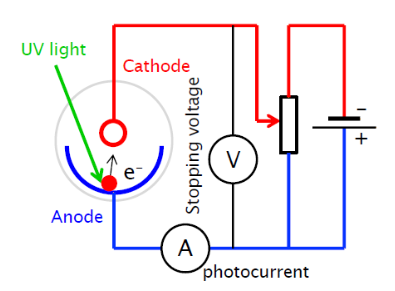
\includegraphics{figures/lec03-01.png}
     \caption{A circuit diagram for measuring the photoelectric effect.}
\end{figure}

The above setup would be encased in a glass ball (containing a vacuum), with a setup like this:

\begin{figure}[H]
    \centering
    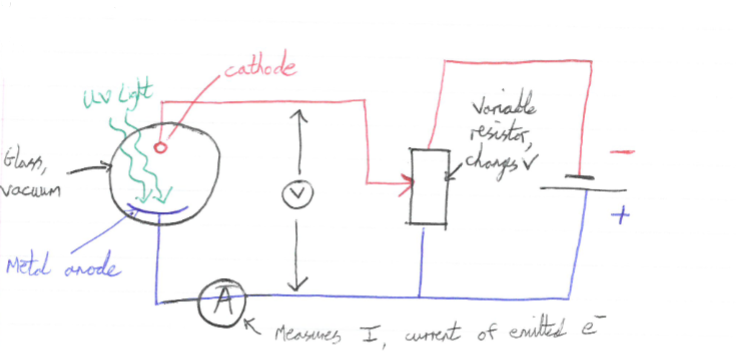
\includegraphics[width=0.75\textwidth]{figures/lec03-02.png}
     \caption{Experimental Setup}
\end{figure}

\subsection*{Results}
\textbf{Result One - Changing Intensity}\\
For fixed UV wavelength, increasing the intensity of light increases the measured photocurrent:
\begin{figure}[H]
    \centering
    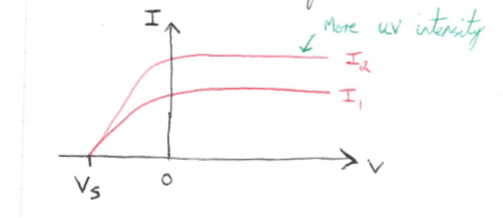
\includegraphics{figures/lec03-03.png}
    \caption{}
\end{figure}
\begin{itemize}
    \item Increasingly negative potential the cathode decreases photocurrent. At some potential $v_s$ (the ``stopping potential'') this current drops to zero.
    \item Potential does not affect electron emission, however adding potential causes an electric field which effectively blows electrons back towards the anode. The stopping potential is when this electric field is perfectly strong to prevent electrons from reaching the cathode and causing a current.
    \item The fact this can happen consistently (i.e. no current means no electrons made it through) implies that there must be some maximum kinetic energy these electrons can have ($KE_{max} = eV_S$).
    \item The stopping potential is independant of UV intensity. More UV makes current increase, but does not change stopping potential (i.e. it does not give more energy to each electron, they each have the same energy). This does not make sense classically. Classically we would expect adding more energy to cause emitted electrons to have more energy, therefore changing the stopping potential.
\end{itemize}

\textbf{Result Two - Changing Wavelength}
\begin{figure}[H]
    \centering
    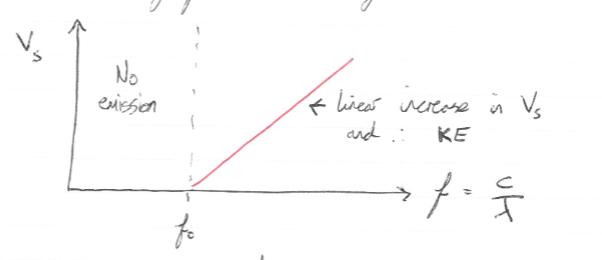
\includegraphics{figures/lec03-04.png}
    \caption{}
\end{figure}

We have to reach some baseline threshold frequency $f_0$ before we see any photocurrent. After this, increasing wavelength increases photocurrent (and hence KE of emitted electrons) linearly.

\begin{itemize}
    \item For a given metal, we find the threshold frequency $f_0$, below which there is no emission of electrons (no current). If below the frequency $f_0$, intensity is irrelevant. This contradicts classical mechanics which would suggest that turning up the light intensity would supply more (and potentially sufficient) energy.
    \item Above the threshold, the energy of individual emitted photons depends on UV frequency and not intensity (by result one).
\end{itemize}

\subsection*{Conclusions}

\textbf{Classically}

Classically, we expect energy to be proportional to intensity, $\therefore$ $v_s$ should increase with greater intensity. We also expect there to be no link between between frequency and energy, hence no threshold frequency. We'd expect no threshold frequency, instead being a time delay as electrons ``soak up'' energy to reach the required threshold.

In theory, great, in practice \emph{this is not observed.}

\textbf{Einstein's Proposal}

Energy in light comes from phots with energy $E = hf$. There is a minimum energy required for an electron to be able to escape from the metal. This minimum energy is called the work function $\phi$.
\[
    KE_\text{max} = hf - \phi = eV_s
\]

Now:
\begin{itemize}
    \item Higher intensity means more of the same particles (more photons), but the energy of each is unchanged.
    \item $E = hf$ so frequency changes energy (as observed).
    \item The Bohr model says that an electron can only have certain electron energy transitions when the correct energy is supplied (an electron cannot gradually soak up energy). This explains why there is a cutoff below the work function, and no observed time delay (as the ``soaking up'' that casues the delay does not happen). Either an incoming photon has sufficient energy, or it does not. Having more photons does not help.
    \item The first incoming photons immediately releases an electron (assuming the incoming light has sufficient energy), therefore there's no time delay.
\end{itemize}

\subsection*{In Practice}
\begin{figure}[H]
    \centering
    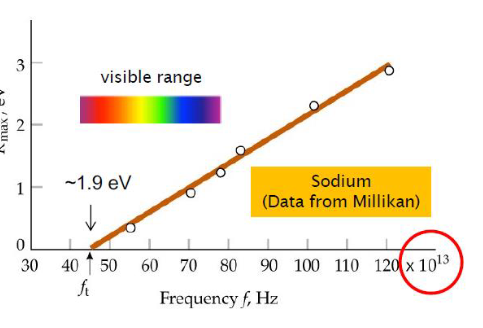
\includegraphics{figures/lec03-05.png}
     \caption{Sodium photocurrent measurements by Robert Millikan}
\end{figure}


\section*{Compton Scattering}
Compton Scattering is the scattering of x-rays off carbon atoms.

\begin{figure}[H]
    \centering
    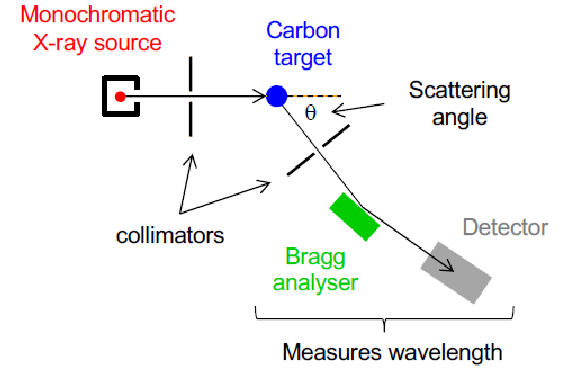
\includegraphics{figures/lec03-06.png}
     \caption{A Compton Scattering experimental setup.}
\end{figure}

The surprising result is that two wavelengths were observed (not just the original) - $\lambda_1, \lambda_2$, where $\lambda_1$ is the original and $\lambda_2$ is different. Classically this is hard to exlain and $\lambda$ should not change.

The difference between these two wavelengths increases with scattering angle $\theta$. This can be explained if the x-ray beam is a stream of photons, but not classically.

Possible options when a photon collides:
\begin{itemize}
    \item Elastic: No loss of energy, hence no change in wavelength.
    \item Inelastic: Change of energy, so the wavelength also changes. An electron is fired out of the target, carrying energy and momentum, so the photon loses energy.
\end{itemize}

\begin{figure}[H]
    \centering
    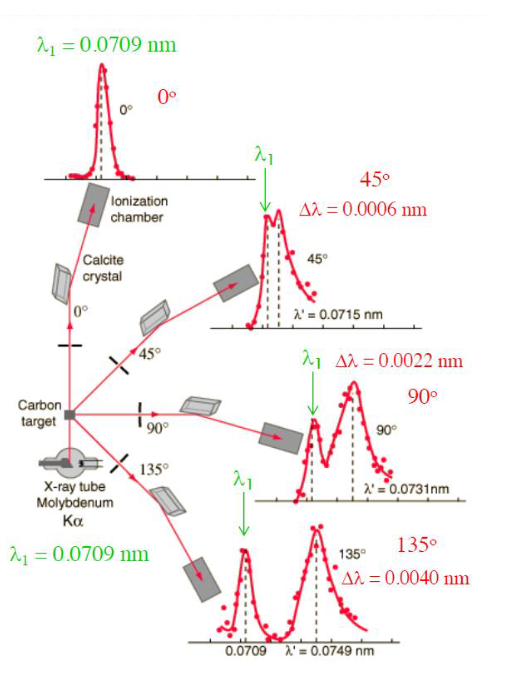
\includegraphics{figures/lec03-07.png}
     \caption{The observed results}
\end{figure}

\section*{Deriving Compton's Equation}
Given an incoming photon with with energy $E_1$, wavelength $\lambda_1$ and momentum $\underline{p}_1$. This strikes a carbon atom and is deflected by angle $\theta$. There is also an emitted electron at angle $\phi$ which must be in the oppsite direction (angled up vs down) to conserve momentum. The new deflected photon has $E_2$, $\lambda_2$, $\underline{p}_2$.

We must consider relativistic effects here given the high speed ($E^2 = p^2c^2 + m^2c^4$)

\begin{figure}[H]
    \centering
    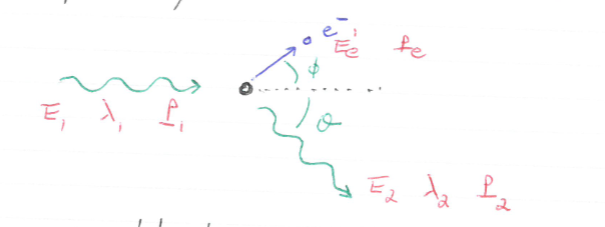
\includegraphics{figures/lec03-08.png}
     \caption{}
\end{figure}

\subsection*{Setup}
For a massless photon ($m = 0$):
\[
    E = pc
\]
And:
\[
    E = \frac{hc}{\lambda}
\]

So:
\begin{equation}
    p = \frac{h}{\lambda}
    \label{cscattere2}
\end{equation}

\subsection*{Conservation and Relativity}
Conserving momentum (underlines ommitted for speed):
\[
    p_1 = p_e + p_2
\]
\[
    p_e = p_1 - p_2
\]

Squaring both sides:
\[
    p_e^2 = p_1^2 + p_2^2 - 2p_1 \cdot p_2
\]
\begin{equation}
    p_e^2 = p_1^2 + p_2^2 - 2p_1p_2 \cos \theta
    \label{cscattere1}    
\end{equation}

And then by conservation of energy:
\[
    E_1 + E_e = E_2 + E_e'
\]

Where $E_1$ is the incoming photon energy, $E_e$ is the energy of the electron at rest in atom before collision, $E_2$ is the deflected photon energy and finally $E_e'$ is the deflected electron's energy.

Using this:
\[
    p_1c + m_e c^2 = p_2 c + \sqrt{p_e^2c^2 + m_e^2c^4}
\]
\[
    \implies p_1 - p_2 + m_ec = \sqrt{p_e^2 + m_e^2c^2}
\]

And squaring both sides:
\[
    (p_1 - p_2)^2 + \cancel{m_e^2c^2} + 2m_ec(p_1 - p_2) = p_e^2 + \cancel{m_e^2c^2}
\]

Subsituting in Eqn \ref{cscattere1} for $p_e^2$
\begin{align*}
    (p_1 - p_2)^2 + 2m_ec(p_1 - p_2) &= p_e^2\\
    (p_1 - p_2)^2 + 2m_ec(p_1 - p_2) &= p_1^2 + p_2^2 - 2p_1p_2 \cos \theta
\end{align*}

And rearranging:
\begin{align*}
    (p_1 - p_2)^2 + 2m_ec(p_1 - p_2) &= p_1^2 + p_2^2 - 2p_1p_2 \cos \theta\\
    p_1^2 + p_2^2 - 2p_1p_2 + 2m_ec(p_1 - p_2) &= p_1^2 + p_2^2 - 2p_1p_2 \cos \theta\\
    -2p_1p_2 + 2m_ec(p_1 - p_2) &= - 2p_1p_2 \cos \theta\\
    -p_1p_2 + m_ec(p_1 - p_2) &= - p_1p_2 \cos \theta\\
    m_ec(p_1 - p_2) &= - p_1p_2 \cos \theta + p_1p_2\\
    m_ec(p_1 - p_2) &= p_1p_2 (1 - \cos \theta) 
\end{align*}

Subsituting Eqn \ref{cscattere2}:
\begin{align*}
    m_ec(p_1 - p_2) &= p_1p_2 (1 - \cos \theta)\\
    m_ec\left(\frac{h}{\lambda_1} - \frac{h}{\lambda_2}\right) &= \frac{h}{\lambda_1} \frac{h}{\lambda_2} (1 - \cos \theta)\\
    m_ec\left(\frac{h}{\lambda_1} - \frac{h}{\lambda_2}\right) &= \frac{h^2}{\lambda_1 \lambda_2} (1 - \cos \theta)\\
    m_ec\left(\frac{1}{\lambda_1} - \frac{1}{\lambda_2}\right) &= \frac{h}{\lambda_1 \lambda_2} (1 - \cos \theta)\\
    m_ec\left(\frac{\lambda_1 \lambda_2}{\lambda_1} - \frac{\lambda_1 \lambda_2}{\lambda_2}\right) &= h (1 - \cos \theta)\\
    m_ec\left(\lambda_2 - \lambda_1\right) &= h (1 - \cos \theta)\\
    \left(\lambda_2 - \lambda_1\right) &= \frac{h}{m_ec} (1 - \cos \theta)
\end{align*}

Which is the Compton Equation. This shows that the change in wavelength is proportional to $1 - \cos \theta$.

\section*{Conclusions}
The photoelectric effect and Compton scattering are two more physical phenomena that cannot be explained using traditional classical mechancics with EM waves alone. They both require assuming photons of energy $E = hf$ to be adequately explained.